\documentclass{article}

\usepackage[authoryear]{natbib}
\usepackage{url}
\usepackage{graphicx}

\title{Assignment 1 Regular Expression}
\author{Wordh Ul Hasan, 133 0471 642}
\date{}

\begin{document}
\maketitle
 

\section{}

\subsection{}
ANSWER TO QUESTION 1(a)

The DFA accepts all the  Binary Strings that ends with 1.

The DFA accepts strings for example 01, 001, 00101, 00111, 1, 111

The DFA Rejects all the strings as 010, 0010, 10, 0, 001110, 1110

\subsection{}


ANSWER TO QUESTION 1(b)


The DFA accepts all the Strings that takes a, b , c as input and contains ba as substring.

The DFA accepts strings for example abcbbaa, abac, cbab, cbcbbac

The DFA Rejects all the strings as abbc, abcaabc, abcbb, abccbb
%%% 

\section{State Diagram}

\subsection{}

YOUR ANSWER TO QUESTION 2(a)

Figure \ref{fig:even_a} shows DFA that accepts only even number of a's in the string
\begin{figure}
  \includegraphics[width=\linewidth]{even_a.JPG}
  \caption{A DFA that accepts only even number of a's}
  \label{fig:even_a}
\end{figure}

\subsection{}

YOUR ANSWER TO QUESTION 2(b)

Figure \ref{fig:even_a_odd_b} shows DFA that accepts only even number of a's and odd number of b's in the string
\begin{figure}
  \includegraphics[width=\linewidth]{even_a_odd_b.JPG}
  \caption{A DFA that accepts only even number of a's and odd num of b's}
  \label{fig:even_a_odd_b}
\end{figure}

\subsection{}

YOUR ANSWER TO QUESTION 2(c)


Figure \ref{fig:startswith_aa_endswith_bb} shows A DFA that accepts all the strings that starts with aa and ends with bb
\begin{figure}
  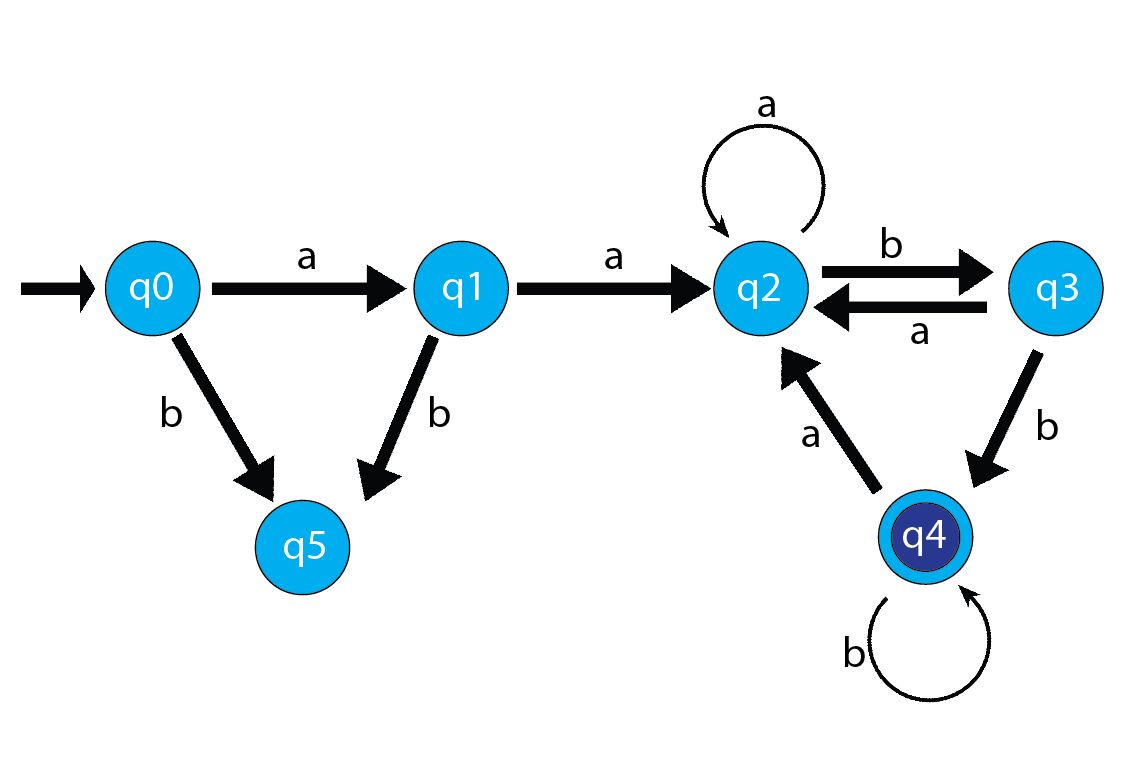
\includegraphics[width=\linewidth]{startswith_aa_endswith_bb.JPG}
  \caption{A DFA that accepts all the strings that starts with aa and ends with bb}
  \label{fig:startswith_aa_endswith_bb}
\end{figure}


\section{Regular Expression from Part 2} 

\subsection{}
YOUR ANSWER TO QUESTION 3(a)

\[(b*ab*ab*)*\]

\subsection{}
YOUR ANSWER TO QUESTION 3(b)

\[(aa|bb)*((ab|ba)(aa|bb)*(ab|ba)(aa|bb)*b)*\]


\subsection{}
YOUR ANSWER TO QUESTION 3(c)

\[aa(a|b)*bb\]

\section{NFA} 

\subsection{}
YOUR ANSWER TO QUESTION 4(a)

Figure \ref{fig:aaa} All strings over {a,b} that have an a as one of the last 3 characters in the string.
\begin{figure}
  \includegraphics[width=\linewidth]{aaa.JPG}
  \caption{A NFA that accepts all the strings that starts with aa and ends with bb}
  \label{fig:aaa}
\end{figure}


\subsection{}
YOUR ANSWER TO QUESTION 4(b)

Figure \ref{fig:aaa} All strings over {E, G, L, O, X} that contain the regular expression GO*GLE.
\begin{figure}
  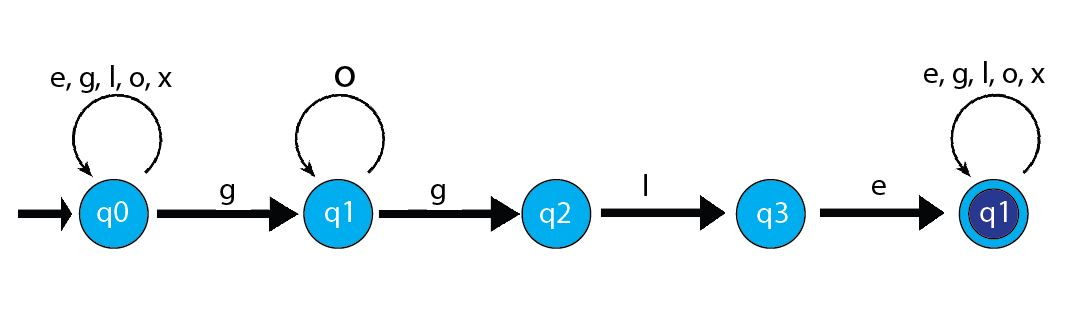
\includegraphics[width=\linewidth]{google.JPG}
  \caption{ an NFA that Accepts All strings over {E, G, L, O, X} that contain the regular expression GO*GLE.}
  \label{fig:google}
\end{figure}


\section{DFA constructed from NFA from 4} 

\subsection{}
YOUR ANSWER TO QUESTION 5(a)

Figure \ref{fig:bdfa} A DFA of All strings over {a,b} that have an a as one of the last 3 characters in the string.
\begin{figure}
  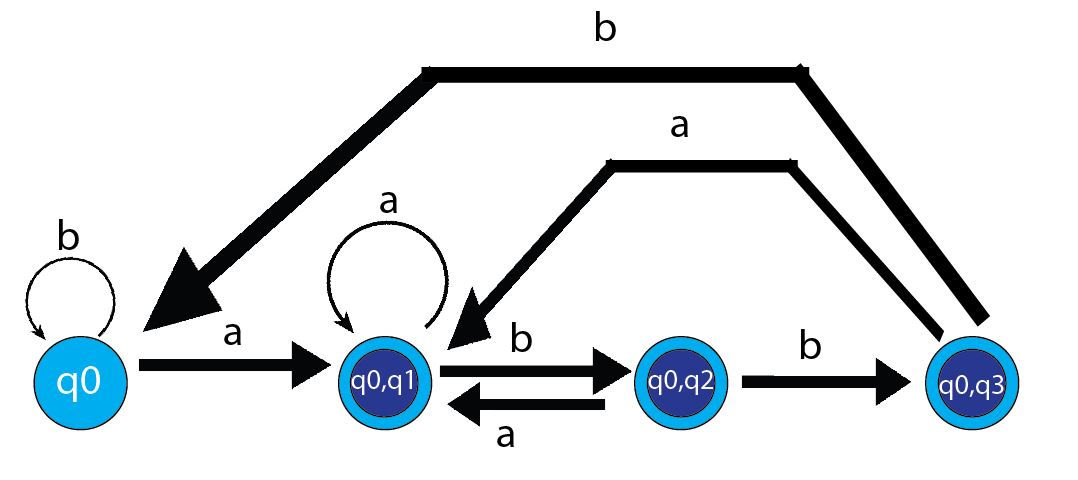
\includegraphics[width=\linewidth]{bdfa.JPG}
  \caption{ An DFA that is constructed from All strings over {a,b} that have an a as one of the last 3 characters in the string.}
  \label{fig:bdfa}
\end{figure}

\subsection{}
YOUR ANSWER TO QUESTION 5(b)

Figure \ref{fig:googledfa} A DFA of All strings over {E, G, L, O, X} that contain the regular expression GO*GLE.
\begin{figure}
  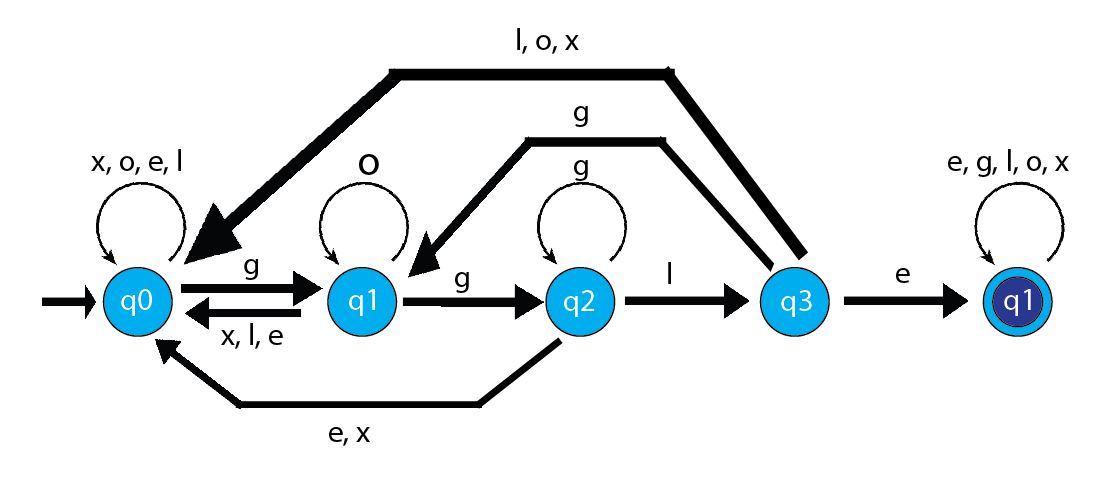
\includegraphics[width=\linewidth]{googledfa.JPG}
  \caption{ an DFA that is constructed from the NFA that Accepts All strings over {E, G, L, O, X} that contain the regular expression GO*GLE.}
  \label{fig:googledfa}
\end{figure}

%%END YOUR PART
\bibliographystyle{chicago}


\end{document}



